\documentclass{article}

% Language setting
% Replace `english' with e.g. `spanish' to change the document language
\usepackage[english]{babel}
\usepackage{cite}
% Set page size and margins
% Replace `letterpaper' with `a4paper' for UK/EU standard size
\usepackage[letterpaper,top=2cm,bottom=2cm,left=3cm,right=3cm,marginparwidth=1.75cm]{geometry}

% Useful packages
\usepackage{amsmath}
\usepackage{graphicx}
\usepackage[colorlinks=true, allcolors=blue]{hyperref}

\title{MapReduce Introduction and Implementation}
\author{Zifan WANG, Yazhou SHEN}

\begin{document}
\maketitle

\begin{abstract}


MapReduce \cite{dean2008mapreduce} is one of the most popular programming model that developed by Google ten years ago. It utilized map and reduce function and take $<key, value>$ pair as input and 
output to get closer to the final result step by step. All programs written in that specific style can run distributed and parallel through MapReduce framework. Parallellization of the framework accelerate the 
execution while distribution make the framework scalable and can handle infinite number of data as long as we have enough machines.

We go through paper that introduce MapReduce as well as papers that gives a clear definition of MapReduce class and proves the correctness of the MapReduce in order to gain a deep understanding of this framework.
We also utilize socket programming to build our own MapReduce framework in python and evaluate its throughput.




\end{abstract}

\section{Introduction}
We are currently in an information explosive era. Large volume of data need to be processed day by day. Computation power is much more valuable than ever. And due to physics limit, people cannot keep reducing the size of semi-conductors' size and Moore Law cannot always be true. Therefore
the computational power of single machine cannot be improved forever. As a result, people need to pay more attenttion
on multiple machine computation system that multiple nodes coordinate with each other to finish the same job. MapReduce, developed by Google, is designed to process large volumn of data. There are mainly three steps in MapReduce framework including: Map, Reduce, Shuffle. Basically each round of Map to Shuffle to Reduce will be 
a simple computation and users can get final result from original input after multiple rounds of simple execution.

\section{Programming Model}
There are two main functions in MapReduce framework: Map
and Reduce. Shuffle part is between Map and Reduce phase that do some intermediate data process.
Map function  take an input pair, and process on it to generate a set
of intermediate $<key, value>$ pairs. The Shuffle function groups the generated
$<key, value>$ pairs altogether by the same key, and passes them to the Reduce
function. Then for the Reduce function, it receives an intermediate key I and a
set of values for that key. Then it merges these values to form smaller set of
values. The Map and Reduce functions are defined
by users, so it is actually highly customizable, as long as it still follows the basic
paradigm.
\section{Structure}
\begin{figure}
      \centering
      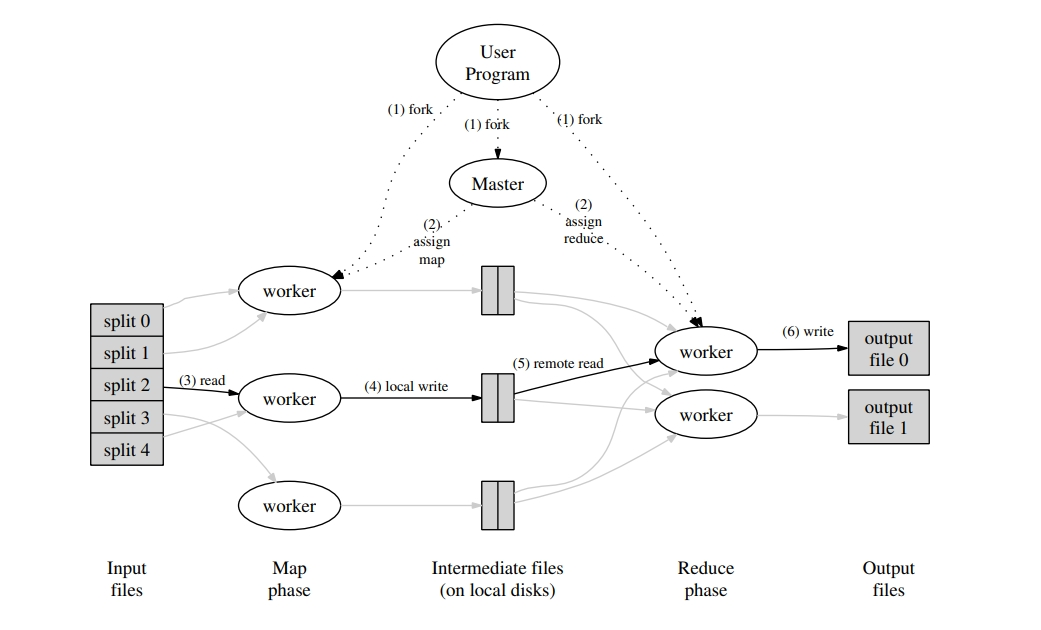
\includegraphics[scale = 0.4]{structure.png}
      \caption{MapReduce Structure \cite{dean2008mapreduce}}
\end{figure}
\subsection{Execution Overview}
The Map invocations are distributed across multiple
machines by automatically partitioning the input data
into a set of M splits. The input splits can be processed in parallel by different machines. Reduce invocations are distributed by partitioning the intermediate key
space into R pieces using a partitioning function (e.g.,
hash(key) mod R). The number of partitions (R) and
the partitioning function are specified by the user.
Figure 1 shows the overall flow of a MapReduce operation in our implementation. When the user program
calls the MapReduce function, the following sequence
of actions occurs (the numbered labels in Figure 1 correspond to the numbers in the list below
\begin{enumerate}
      \item The MapReduce library in the user program first
      splits the input files into M pieces of typically 16
      megabytes to 64 megabytes (MB) per piece (controllable by the user via an optional parameter). It
      then starts up many copies of the program on a cluster of machines.
      \item One of the copies of the program is special - the
      master. The rest are workers that are assigned work
      by the master. There are M map tasks and R reduce
      tasks to assign. The master picks idle workers and
      assigns each one a map task or a reduce task.
      \item A worker who is assigned a map task reads the
      contents of the corresponding input split. It parses
      key/value pairs out of the input data and passes each
      pair to the user-defined Map function. The intermediate key/value pairs produced by the Map function
      are buffered in memory
      \item  Periodically, the buffered pairs are written to local
      disk, partitioned into R regions by the partitioning
      function. The locations of these buffered pairs on
      the local disk are passed back to the master, who
      is responsible for forwarding these locations to the
      reduce workers.
      \item When a reduce worker is notified by the master
      about these locations, it uses remote procedure calls
      to read the buffered data from the local disks of the
      map workers. When a reduce worker has read all intermediate data, it sorts it by the intermediate keys
      so that all occurrences of the same key are grouped
      together. The sorting is needed because typically
      many different keys map to the same reduce task. If
      the amount of intermediate data is too large to fit in
      memory, an external sort is used.
      \item The reduce worker iterates over the sorted intermediate data and for each unique intermediate key encountered, it passes the key and the corresponding
      set of intermediate values to the user's Reduce function. The output of the Reduce function is appended
      to a final output file for this reduce partition.
      \item When all map tasks and reduce tasks have been
      completed, the master wakes up the user program.
      At this point, the MapReduce call in the user program returns back to the user code.
\end{enumerate}
\subsection{How to add Comments and Track Changes}

Comments can be added to your project by highlighting some text and clicking ``Add comment'' in the top right of the editor pane. To view existing comments, click on the Review menu in the toolbar above. To reply to a comment, click on the Reply button in the lower right corner of the comment. You can close the Review pane by clicking its name on the toolbar when you're done reviewing for the time being.

Track changes are available on all our \href{https://www.overleaf.com/user/subscription/plans}{premium plans}, and can be toggled on or off using the option at the top of the Review pane. Track changes allow you to keep track of every change made to the document, along with the person making the change. 

\subsection{Fault Tolerance}

Fault tolerance is an important part in MapReduce framework since we need to deal with a large number of cluster. 


\subsection{How to write Mathematics}

\LaTeX{} is great at typesetting mathematics. Let $X_1, X_2, \ldots, X_n$ be a sequence of independent and identically distributed random variables with $\text{E}[X_i] = \mu$ and $\text{Var}[X_i] = \sigma^2 < \infty$, and let
\[S_n = \frac{X_1 + X_2 + \cdots + X_n}{n}
      = \frac{1}{n}\sum_{i}^{n} X_i\]
denote their mean. Then as $n$ approaches infinity, the random variables $\sqrt{n}(S_n - \mu)$ converge in distribution to a normal $\mathcal{N}(0, \sigma^2)$.


\subsection{How to change the margins and paper size}

Usually the template you're using will have the page margins and paper size set correctly for that use-case. For example, if you're using a journal article template provided by the journal publisher, that template will be formatted according to their requirements. In these cases, it's best not to alter the margins directly.

If however you're using a more general template, such as this one, and would like to alter the margins, a common way to do so is via the geometry package. You can find the geometry package loaded in the preamble at the top of this example file, and if you'd like to learn more about how to adjust the settings, please visit this help article on \href{https://www.overleaf.com/learn/latex/page_size_and_margins}{page size and margins}.

\subsection{How to change the document language and spell check settings}

Overleaf supports many different languages, including multiple different languages within one document. 

To configure the document language, simply edit the option provided to the babel package in the preamble at the top of this example project. To learn more about the different options, please visit this help article on \href{https://www.overleaf.com/learn/latex/International_language_support}{international language support}.

To change the spell check language, simply open the Overleaf menu at the top left of the editor window, scroll down to the spell check setting, and adjust accordingly.

\subsection{How to add Citations and a References List}

You can simply upload a \verb|.bib| file containing your BibTeX entries, created with a tool such as JabRef. You can then cite entries from it, like this: \cite{greenwade93}. Just remember to specify a bibliography style, as well as the filename of the \verb|.bib|. You can find a \href{https://www.overleaf.com/help/97-how-to-include-a-bibliography-using-bibtex}{video tutorial here} to learn more about BibTeX.

If you have an \href{https://www.overleaf.com/user/subscription/plans}{upgraded account}, you can also import your Mendeley or Zotero library directly as a \verb|.bib| file, via the upload menu in the file-tree.

\subsection{Good luck!}

We hope you find Overleaf useful, and do take a look at our \href{https://www.overleaf.com/learn}{help library} for more tutorials and user guides! Please also let us know if you have any feedback using the Contact Us link at the bottom of the Overleaf menu --- or use the contact form at \url{https://www.overleaf.com/contact}.

\bibliographystyle{IEEEtran}
\bibliography{IEEEexample}

\end{document}